%%%%%%%%%%%%%%%%%%%%%%%%%%%%%%%%%%%%%%%%%%%%%%%%%%%%%%%%%%%%%%%%%%%
%                                                                 %
%  GEANT manual in LaTeX form                              %
%                                                                 %
%  Michel Goossens (for translation into LaTeX)                   %
%  Version 1.00                                                   %
%  Last Mod. Jan 24 1991  1300   MG + IB                          %
%                                                                 %
%%%%%%%%%%%%%%%%%%%%%%%%%%%%%%%%%%%%%%%%%%%%%%%%%%%%%%%%%%%%%%%%%%%
\Origin{R.Brun}
\Submitted{01.11.83}     \Revised{18.12.93}
\Version{Geant 3.16}     \Routid{HITS299}
\Makehead{The JHITS data structure}

\begin{figure}[hbt]
     \centering
     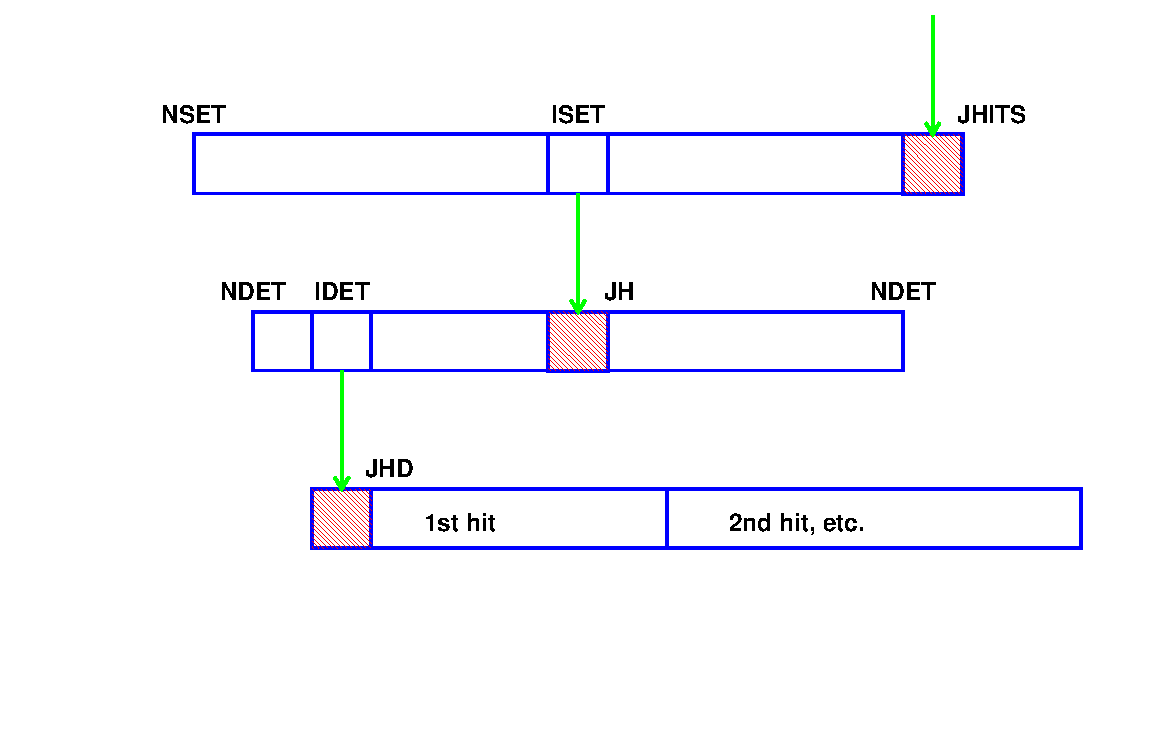
\epsfig{file=eps/hits299-1.eps,width=14cm}
     \caption{Layout of the {\tt JHITS} data structure}
     \label{fg:hits299-1}
\end{figure}

\begin{tabular}{lp{12cm}}
\tt JH=LQ(JHITS-ISET) & pointer to hits structure for set number {\tt ISET} \\
\tt IQ(JH+IDET) & number of words used for storing the hits
of detector number {\tt IDET} \\
\tt JHD=LQ(JH-IDET) & pointer to hits bank for detector number {\tt IDET} of
set number {\tt ISET} \\
\tt IQ(JHD+1) & 1$^{st}$ word of 1$^{st}$ hit \\
\tt IQ(JHD+NWH+1) & 1$^{st}$ word of 2$^{nd}$ hit \\
\tt JS=LQ(JSET-ISET) & pointer to the structure containing the description
of set number {\tt ISET} \\
\tt JD=LQ(JS-IDET) & pointer to the bank containing the description of detector
number {\tt IDET} of set number {\tt ISET} \\
\tt NWH=IQ(JD+3) & number of words in which a hit of detector
number {\tt IDET} of set number {\tt ISET} is stored
\end{tabular}

The {\tt JHITS} structure is filled with the routines \Rind{GSAHIT} and
\Rind{GSCHIT}.
The routine \Rind{GFHITS} can be used to get the hits for a detector
{\tt IDET} in set {\tt ISET}.
